 %===================================== CHAP 5 =================================

\chapter{Architecture and implementation, Not finished}
\label{ch:architecture_and_implementation}

This chapter explains the processes and solutions made in the design phase of the solution. It also explains the actual implementation of the system.

\section{User interface}
\label{sec:architecture_and_implementation-user_interface}

One of the initial requirements from the customer, was to have a graphical user interface. It was supposed to display relevant data and allow the administrator to moderate topics and subscriptions. After an initial consideration, the Spring Framework\footnote{\url{http://projects.spring.io/spring-boot/}} was chosen to be the most suitable (see section \ref{subsec:prestudies-tools-spring_mvc}) for the administration panel. The user interface is implemented using the MVC-pattern. 

\subsection{Design}
\label{subsec:architecture_and_implementation-user_interface-design}

Since the group spent a considerable amount time researching the Apollo broker during the research phase, it had gained a lot of insight regarding what an administration panel should contain. Originally the customer had not stated any specific requirements for the administration panel. Therefore, an initial sketch was created, and discussed with the customer. The sketch was heavily influenced by Apollo. This sketch (figure \ref{fig:initial_prototype}), along with the creation of use cases, set the terms for creating a prototype.

The group agreed upon creating a functional prototype for the customer. This prototype was made available, so that the customer could provide feedback. During all customer meetings the group discussed the current version of the administration panel with the customer. This discussions gave feedback on how new elements in the panel met the customers expectations. This approach gave the group one big advantage; rapid response from the customer which made it easy to improve the interface and add additional features. So throughout the lifetime of the development phase the administration panel where continuously released and deployed on our test server after each sprint.

The final interface contains of five panes; "Main", "Topics", "Statistics", "Logs" and "Configuration". The "Main"-pane contains information about the message broker. The "Main"-pane is meant to give a general overview of the current operating environment, as well as the system status. The "Statistics"-pane contain useful statistics about requests, messages etc. on the different protocols. Also, it shows general usage of the memory. The "Logs"-pane contains runtime logs for debugging purposes. The "Topics"-pane shows all registered topics in the message broker. In this pane, information about the current topics and subscriptions is available, as well as the possibility to remove topics and subscribers. Finally, in the "Configuration"-pane, the user can change the brokers settings and map topics together.

\begin{center}
  \begin{figure}[ht!]
    \makebox[\textwidth]{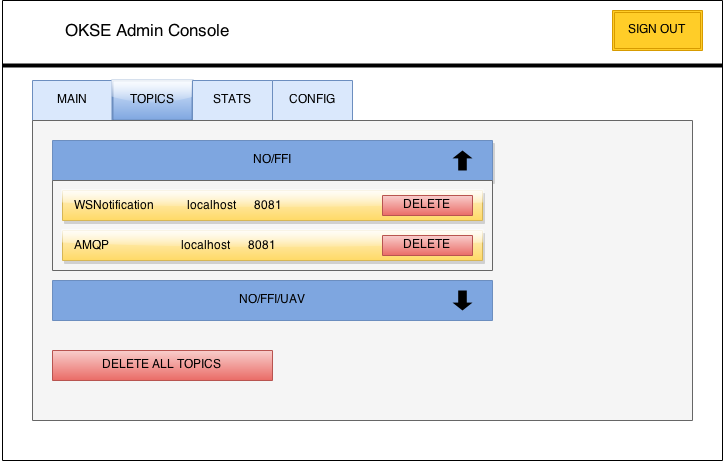
\includegraphics[scale=0.5]{fig/initial_prototype.png}}
    \caption{Admin interface functional prototype}
    \label{fig:initial_prototype}
  \end{figure}
\end{center}

\subsection{Implementation}
\label{subsec:architecture_and_implementation-implementation}

The front-end was designed in a modularized way, where one controller class was responsible for one pane. The main argument for this approach was the idea of having the administration panel designed as a single page web application. The page uses AJAX-requests to reach a representational state transfer (hereby denoted as REST) API. By using the Spring Framework, the system exposes API-endpoints which can be used to access and/or modify data. This is used as the main data source for the front-end and is a critical part of the single page design. Translated to the MVC-pattern, the Spring Framework works as a controller through REST-controllers. Furthermore the different panes act out as views. Each AJAX-request to the API-endpoints will reach the controllers and modify the models and/or message broker. Structuring the system this way gave some advantages: 

\begin{itemize}
    \item No need for refresh of the entire administration panel
    \item One controller class served one pane; easy to debug
    \item Loose coupling, no dependency between panes
    \item Easy to extend the application further.
\end{itemize}

\subsubsection{Architecture}

\begin{center}
  \begin{figure}[ht!]
    \makebox[\textwidth]{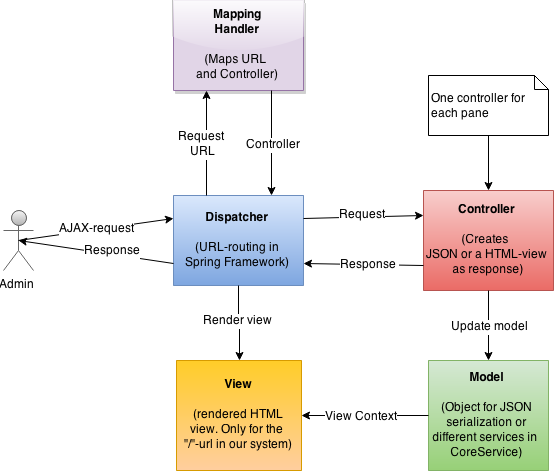
\includegraphics[scale=0.5]{fig/spring.png}}
    \caption{REST-API architecture}
    \label{fig:spring}
  \end{figure}
\end{center}

Figure \ref{fig:spring} shows an overview on how a request is handled in the server. The main workflow is as follows:

\begin{itemize}
    \item\textbf{Dispatcher} -  This is the class that is exposed to the user. It forwards the request URL to the mapping handler to get the correct controller. Then it calls the controller responsible for the request. Finally it returns the response to the user. 
    \item\textbf{Mapping handler} - This class maps the request URL to the controller responsible for the request and returns it to the dispatcher. 
    \item\textbf{Controller} - This is the class responsible for executing tasks and getting information from the message broker. It returns a response JSON to the dispatcher.  
\end{itemize}

\section{Broker architecture}
\label{sec:architecture_and_implementation-broker_architecture}

This section discusses the high-level aspects taken into consideration when designing the broker architecture. Some parts of the system may be explained in greater detail to provide clear purpose or intent.

\subsection{Goals and strategy}
\label{subsec:architecture_and_implementation-goals_and_strategy}

Building on the results and findings in the research phase, the team created a set of goals for the design of the system architecture. Several aspects of the Apollo broker were really well thought out, and were on the priority list from the start. These included, but were not limited to: Completely protocol agnostic interface. A priority message queue, supported by a multi-threaded execution service. Loose coupling of modules. High extendability, and low maintenance effort.

Expanding on these traits, the group wanted a system architecture where each component was a standalone service. A service would expose a public interface from which other components could request data access or services from. Another goal of the design was to have a core service responsible for registering other services, starting them, stopping them, and registering protocols. This would allow extending of the system by simply registering the new component, without further modifications.

The customer had requested a graphical user interface, and building on the experience and knowledge in the group, a web based interface was deemed most appropriate. The group wanted to have an administration interface built using the dynamic properties of the outlined system. Registering a new protocol should not require the administration interface component to be modified. Registering a new core service that a potential developer wanted to expose in the admin interface should only require adding a new model, API controller and template fragment.

Based on these thoughts and ideas, a list of goals was created:

\begin{itemize}
\item The system should not need to know about the details of registered protocols in order to perform as intended. In essence, it should be completely protocol agnostic.
\item Extending the system with new functionality should be as easy as possible
\item Extending the system with new protocols should be as easy as possible
\item Extending the system should require as little alteration to existing code as possible
\item Core functionality should be adhering to the principle of "Separation of concerns"
\item Core services should be standalone entities that other components can utilize
\item The system should have a core service responsible for the entire life cycle of other registered components
\end{itemize}

With these goals settled, it was apparent that our design outline had properties of a Service Oriented Architecture\footnote{\url{http://en.wikipedia.org/wiki/Service-oriented_architecture}} (hereby denoted as SOA), as well as the Module Pattern\footnote{\url{http://en.wikipedia.org/wiki/Module_pattern}}. This prompted that the actual implementation of the system should adhere to these principles and patterns as much as possible, for consistency and future familiarity.

Putting all this together, a high-level system architecture was created (fig \ref{fig:abstract_architecture}). It illustrates the main entities that were to become the brokering system. Lines between entities illustrate their connection to the core service responsible for all other entity life cycles. Yellow entities are core services in the brokering system, while black are protocol components.

\begin{center}
  \begin{figure}[ht!]
    \makebox[\textwidth]{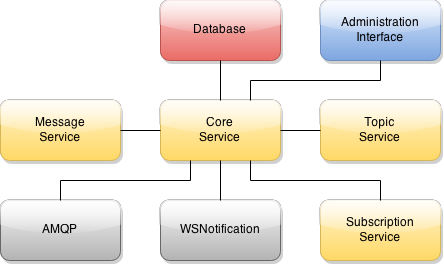
\includegraphics[scale=0.6]{fig/abstract_architecture.png}}
    \caption{High-level system architecture}
    \label{fig:abstract_architecture}
  \end{figure}
\end{center}

The next step was to identify functional dependencies and usage dependencies between the components in the system. 

\section{Implementation}
\label{sec:architecture_and_implementation-implementation}

\subsection{WSN}
\label{subsec:architecture_and_implementation-implementation-wsn}

Here be information about how WSN was implemented, as well as how it works

\subsection{AMQP}
\label{subsec:architecture_and_implementation-implementation-amqp}

Here be information about how AMQP was implemented, as well as how it works

\clearpage

\section{Message workflow}
\label{sec:architecture_and_implementation-message_workflow}

\begin{center}
  \begin{figure}[ht!]
    \makebox[\textwidth]{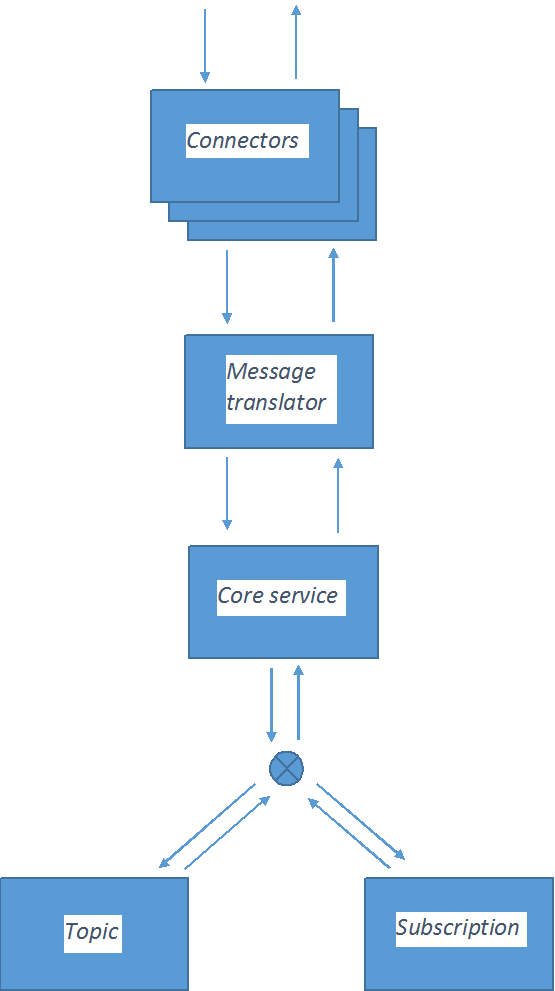
\includegraphics[scale=0.3]{fig/MessageWorkflow.png}}
    \caption{Message workflow}
    \label{fig:Message workflow}
  \end{figure}
\end{center}

\clearpage